\documentclass[11pt,a4paper]{article}
\usepackage[margin=1in]{geometry}
\usepackage{booktabs}
\usepackage{graphicx}
\usepackage{listings}
\usepackage{xcolor}
\usepackage{float}
\usepackage{amsmath}
\usepackage{hyperref}
\usepackage{array}
\usepackage{pgfplots}
\pgfplotsset{compat=1.17}
\usepackage{multirow}

\lstset{
  basicstyle=\ttfamily\footnotesize,
  breaklines=true,
  frame=single,
  columns=fullflexible,
  showstringspaces=false
}

\title{\vspace{-1.5em}\textbf{CS683 PA-2}}
\author{
  \begin{tabular}{c@{\hspace{3em}}c}
    \textbf{Abhinav Gupta} & \textbf{Dinesh Methre} \\
    26M2135 & 23B1228 \\[1.2em]
    \textbf{Om Dwivedi} & \textbf{Saravan Kumar} \\
    26M2108 & 23B3922
  \end{tabular}
}
\date{}

\begin{document}
\maketitle
\vspace{-1.5em}

\section{Past Mistakes}

The previous assignment was the first assignment at IIT Bombay for half of the team, and we
made several mistakes that we aim to rectify this time. The key lessons
we have taken forward are:

\begin{itemize}
  \item \textbf{Prioritising the report:} In the previous assignment,
  we spent too much time optimising the code and neglected report
  writing.

  \item \textbf{Using LaTeX:} We used Google Docs for part of the
  previous report and only learned afterwards that reports were
  expected to be written in LaTeX.

  \item \textbf{Understanding data collection:} We used AI to help
  write Bash and Python scripts for collecting experimental data.
  However, we did not sufficiently inspect the available data or
  verify the scripts' behaviour, and ended up trusting the AI too much and missing out on some easy fixes.

  \item \textbf{Writing the report ourselves:} With most of our time
  spent on implementation, we turned to AI to produce a starting point for the report. Correcting its mistakes took
  more time than expected, and some errors still made it into the
  final submission.

  \item \textbf{AI, AI, AI:} Overall, we learned that
  treating AI as a shortcut can create more work than it saves.
  Although eliminating the use of AI would put the team at a disadvantage, we have minimised the use this time.
\end{itemize}

\section{Simulation Configuration}

\begin{figure}
    \centering
    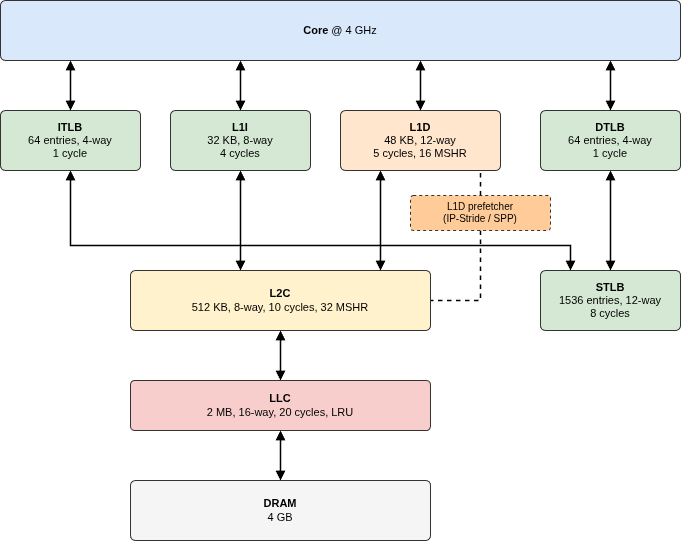
\includegraphics[width=0.75\linewidth]{champsim_system.drawio.png}
    \caption{Champsim Configuration}
    \label{fig:champsim-config}
\end{figure}

All experiments are conducted using the ChampSim simulator. The
simulated system configuration is in
Table~\ref{tab:config}, and the configurations used for our experiments is in Table~\ref{tab:runs}.

\begin{table}[H]
  \centering
  \caption{Champsim Configuration}
  \label{tab:config}
  \begin{tabular}{@{}ll@{}}
    \toprule
    \textbf{Component} & \textbf{Configuration} \\
    \midrule
    Core       & 4\,GHz, out-of-order, 352-entry ROB \\
    L1I        & 32\,KB, 8-way, 4 cycles, LRU \\
    L1D        & 48\,KB, 12-way, 5 cycles, 16 MSHRs, LRU \\
    L2C        & 512\,KB, 8-way, 15 cycles, policy per Table~\ref{tab:runs} \\
    LLC        & 2\,MB, 16-way, 35 cycles, LRU \\
    DRAM       & 4\,GB, 1 channel, 6400\,MT/s \\
    Simulation & 25M warmup + 25M simulated instructions \\
    \bottomrule
  \end{tabular}
\end{table}

\begin{table}[H]
  \centering
  \caption{Experiment Configurations}
  \label{tab:runs}
  \begin{tabular}{@{}lll@{}}
    \toprule
    \textbf{Configuration} & \textbf{L1D prefetcher}
    & \textbf{L2C replacement} \\
    \midrule
    Baseline                   & None & LRU \\
    Task 1A: IP-Stride  & IP-Stride & LRU\\
    Task 1B: SPP                & SPP  & LRU \\
    Task 2A: I-RRIP            & None & I-RRIP \\
    Task 2B: Dynamic I-RRIP    & None & Dynamic I-RRIP \\
    Task 3: SPP + Dynamic I-RRIP
                               & SPP  & Prefetch-aware Dynamic I-RRIP \\
    \bottomrule
  \end{tabular}
\end{table}

\section{Prefetching}

\subsection{Task 1A: Understanding the IP-Stride Prefetcher}

The repository contains a pre-existing implementation of an IP-Stride
prefetcher. An IP-Stride prefetcher records the last memory address
accessed by each LOAD instruction, identified by its instruction
pointer (IP). When the same LOAD executes again, the prefetcher
computes the \textbf{stride} by subtracting the previous address from
the current address. Once the same stride has been observed for a
minimum number of consecutive accesses, the prefetcher becomes
confident in the pattern and issues prefetch requests according to
a configured degree and distance.

\paragraph{IP-Stride in ChampSim}

The default implementation of the IP-Stride prefetcher in ChampSim
(\texttt{prefetcher/ip\_stride.l1d\_pref}) has the following
configuration:

\begin{table}[htbp]
  \centering
  \caption{IP-Stride configuration}
  \label{tab:ip-stride}
  \begin{tabular}{@{}lll@{}}
    \toprule
    \textbf{Configuration} & \textbf{Value} & \textbf{Description} \\
    \midrule
    Tracker entries & 24 & Fully associative, LRU replacement \\
    IP mask & \texttt{0xFF} & Multiple IPs may map to the same entry \\
    Prefetch degree & 3 & Number of prefetch requests \\
    Confidence rule & 2 equal strides & Confidence threshold \\
    Stride unit & Cache line & 64\,B blocks \\
    Page boundary & 4\,KB & Prefetches do not cross page boundaries \\
    Fill level & L1 or L2 & L1 if MSHR occupancy is below 50\%; otherwise L2 \\
    \bottomrule
  \end{tabular}
\end{table}

Each tracker entry stores the masked IP, the last cache-line address
accessed by that IP, the last observed stride, and an LRU counter.
On every L1D load, the prefetcher operates as follows:

\begin{enumerate}
  \item \textbf{Lookup:} The IP is matched against the 24 trackers, and if it does not match the LRU tracker is evicted and the new IP is tracked

  \item \textbf{Stride computation:} On a hit, the stride is computed
  as the difference between the current and previous cache-line
  addresses. If the same cache line is accessed again (stride = 0),
  the access is ignored.

  \item \textbf{Prefetch:} If the stride matches the previously
  recorded stride, prefetches are issued for
  $\text{addr} + k \cdot \text{stride}$, where $k = 1, 2, 3$.
  Prefetching stops at the first address outside the current 4\,KB
  page.

  \item \textbf{Update:} The last address and stride are stored,
  and the entry becomes the most recently used.
\end{enumerate}

\paragraph{Limitations}

This design only captures \emph{uniform} strides. For a repeating
non-uniform pattern such as $(+1, +2, +2, +2, +3)^n$, the IP-Stride
prefetcher cannot learn the complete pattern. It may become confident
in a stride of $+2$ even though the access pattern subsequently changes.
Additionally, the prefetch degree is fixed regardless of how useful
the prefetches are, and masking the IP to 8 bits allows unrelated
loads to alias to the same tracker.



\subsection{Task 1B: Stride Pattern Prefetcher (SPP)}

  The Stride Pattern Prefetcher (SPP) is designed to overcome the
  limitations of the IP-Stride prefetcher. According to the assignment,
  it must:

  \begin{itemize}
    \item \textbf{Track patterns per IP:} maintain a table that records
    the access behaviour of each load instruction.
    \item \textbf{Detect uniform strides:} constant strides such as
    $A, A{+}2, A{+}4, A{+}6, \ldots$
    \item \textbf{Detect non-uniform strides:} repeating multi-stride
    patterns such as $A, A{+}1, A{+}3, A{+}5, A{+}7, A{+}10, A{+}11,
    \ldots$, generated by the stride sequence $(+1, +2, +2, +2, +3)^n$.
    \item \textbf{Signature:} represents the sequence of recently
    observed strides by a signature that maps to the next expected stride.
    \item \textbf{Support a degree greater than 1.}
    \item \textbf{Throttle by accuracy:} measure the usefulness of
    prefetches and scale the degree accordingly to avoid cache pollution.
    \item \textbf{Stay within the page:} never prefetch across a 4\,KB
    page boundary.
  \end{itemize}

  \subsubsection{Design}

  Our SPP consists of three structures: an \textbf{IP table}, a
  \textbf{pattern table}, and an \textbf{accuracy filter}.

  \paragraph{IP table.} A 256-entry direct-mapped table indexed by the
  low 8 bits of the IP. The remaining IP bits are stored as a tag, so
  unrelated loads that share the low 8 bits do not corrupt each other's
  history (unlike the \texttt{0xFF} mask of IP-Stride). Each entry stores
  the last cache line accessed by the IP, its stride, a 2-bit uniform
  confidence counter, and an 8-bit signature of its recent strides.

  \paragraph{Pattern table.} A 256-entry table indexed by the signature.
  Each entry stores the stride that follows that signature (the predicted stride),
  together with a 2-bit confidence counter. The table is shared by all
  IPs, so loops with the same access pattern train the same entries.

  \paragraph{Signature.} After every stride $s$, the signature of the IP
  is updated as
  \[
    \mathit{sig} \leftarrow \big((\mathit{sig} \ll 3) \oplus
    (s \mathbin{\&} \texttt{0x7F})\big) \mathbin{\&} \texttt{0xFF}.
  \]
  Shifting by 3 bits and keeping 8 bits means that each stride influences
  the signature for roughly three subsequent strides, so the signature
  summarises the last three strides. For the pattern
  $(+1, +2, +2, +2, +3)^n$, the signature settles into a cycle of five
  distinct values,
  \[
    82 \xrightarrow{+2} 146 \xrightarrow{+3} 147 \xrightarrow{+1} 153
    \xrightarrow{+2} 202 \xrightarrow{+2} 82,
  \]
  one per position in the pattern, so every signature maps to exactly one
  next stride.

  \paragraph{Training.} On every L1D load, the stride is computed as the
  difference between the current and the previous cache line of the IP.
  A stride of 0 is ignored, and a stride larger than 63 lines (outside
  the page) resets the IP's history. Otherwise:
  \begin{enumerate}
    \item The \emph{uniform confidence} is incremented if the stride
    matches the stored stride, and decremented otherwise. The stored
    stride is only replaced once the confidence has reached 0, so a
    single irregular access does not break a stream.
    \item The pattern table entry of the \emph{previous} signature is
    trained with the observed stride using the same saturating-counter
    rule.
    \item The signature is updated with the new stride.
  \end{enumerate}

 \paragraph{Prefetching.} On every access, the prefetcher decides how to
  generate the strides of the prefetch requests.
  If the uniform confidence is at least 2, the prefetcher uses
  \textbf{uniform mode} and issues $\text{line} + k \cdot \text{stride}$
  for $k = 1 \ldots \text{degree}$. Otherwise it falls back to
  \textbf{pattern mode}: it reads the predicted stride from the pattern
  table, advances the predicted line, updates a copy of the signature with
  the predicted stride, and repeats. This allows the prefetcher to lookahead several steps
  of a non-uniform pattern, for example, at line $A$ with signature 147 and
  degree 4, it issues $A{+}1, A{+}3, A{+}5, A{+}7$. Pattern mode stops as
  soon as a pattern table entry has zero confidence. In both modes,
  prefetching stops at the first line outside the current 4\,KB page. As
  in IP-Stride, a line is filled into L1 if the MSHR is less than half
  full, and into L2 otherwise.

  \paragraph{Accuracy-based throttling.} Every issued prefetch is
  recorded in a 64-entry filter indexed by $\text{line} \bmod 64$ because a $4KB$ page is only 64 lines for a $64B$ cache line. When a
  demand load hits a line present in the filter, the prefetch is counted
  as useful and the entry is cleared. After every 256 issued prefetches
  (one epoch), the accuracy of the epoch is computed and the degree is
  set according to Table~\ref{tab:throttle}.

  \begin{table}[H]
    \centering
    \caption{Accuracy-based degree selection}
    \label{tab:throttle}
    \begin{tabular}{@{}cc@{}}
      \toprule
      \textbf{Epoch accuracy} & \textbf{Degree} \\
      \midrule
      $\geq 75\%$   & 8 \\
      $50$--$75\%$  & 6 \\
      $25$--$50\%$  & 3 \\
      $< 25\%$      & 2 \\
      \bottomrule
    \end{tabular}
  \end{table}

 \subsubsection{Results}

  Table~\ref{tab:spp-results} compares IP-Stride and SPP against the
  baseline without an L1D prefetcher. Speedup is the IPC relative to the
  baseline, accuracy is taken from the ChampSim statistics, and coverage
  is computed as
  \[
    \text{L1D Coverage} =
    \frac{\text{L1D load misses}_{\text{baseline}} -
          \text{L1D load misses}_{\text{prefetcher}}}
         {\text{L1D load misses}_{\text{baseline}}}.
  \]


\begin{table}[htbp]
    \centering
    \caption{IP-Stride and SPP results}
    \label{tab:spp-results}
    \resizebox{\textwidth}{!}{%
    \begin{tabular}{@{}llccccc@{}}
      \toprule
      \textbf{Trace} & \textbf{Prefetcher} & \textbf{IPC} &
      \textbf{Speedup} & \textbf{L1D Load MPKI} &
      \textbf{Accuracy (\%)} & \textbf{Coverage (\%)} \\
      \midrule
      \multirow{3}{*}{Trace 1}
        & None      & 0.2319 & Baseline & 10.68 & --    & --    \\
        & IP-Stride & 0.2328 & 1.0040 & 10.12 & 52.68 & 5.23  \\
        & SPP       & 0.2341 & 1.0093 & 9.38  & 48.00 & 12.15 \\
      \midrule
      \multirow{3}{*}{Trace 2}
        & None      & 0.2513 & Baseline & 13.54 & --    & --    \\
        & IP-Stride & 0.2511 & 0.9992 & 13.44 & 38.23 & 0.74  \\
        & SPP       & 0.2551 & 1.0149 & 12.86 & 43.20 & 5.02  \\
      \midrule
      \multirow{3}{*}{Trace 3}
        & None      & 0.3821 & Baseline & 3.40  & --    & --    \\
        & IP-Stride & 0.3830 & 1.0024 & 3.32  & 15.98 & 2.49  \\
        & SPP       & 0.3905 & 1.0221 & 2.74  & 35.51 & 19.45 \\
      \midrule
      \multicolumn{2}{@{}l}{Geomean speedup}
        & & IP-Stride: 1.0019 & & & \\
      \multicolumn{2}{@{}l}{}
        & & SPP: 1.0154 & & & \\
      \bottomrule
    \end{tabular}%
    }
\end{table}

\begin{figure}[H]
    \centering
    \pgfplotsset{
      sppbars/.style={
        ybar,
        bar width=7pt,
        width=0.49\textwidth,
        height=6.5cm,
        symbolic x coords={Trace 1,Trace 2,Trace 3},
        xtick=data,
        enlarge x limits=0.25,
        nodes near coords,
        every node near coord/.append style={
          font=\tiny,
          rotate=90,
          anchor=west,
          inner sep=1.5pt
        },
        /pgf/number format/fixed,
        /pgf/number format/fixed zerofill,
        /pgf/number format/precision=2,
        /pgf/number format/1000 sep={},
        legend style={
          at={(0.5,-0.14)},
          anchor=north,
          legend columns=-1,
          font=\scriptsize,
          /tikz/every even column/.append style={column sep=6pt}
        },
        ymajorgrids,
        tick label style={font=\scriptsize},
        label style={font=\footnotesize},
        yticklabel style={/pgf/number format/fixed},
        scaled y ticks=false,
        clip=false
      }
    }

    % Speedup
    \begin{tikzpicture}
      \begin{axis}[
        sppbars,
        ylabel={Speedup},
        ymin=0.99,
        ymax=1.045,
        ytick={0.99,1.00,1.01,1.02,1.03,1.04},
        yticklabel style={/pgf/number format/precision=2},
        /pgf/number format/precision=4
      ]
        \addplot coordinates {
          (Trace 1,1.0040)
          (Trace 2,0.9992)
          (Trace 3,1.0024)
        };
        \addplot coordinates {
          (Trace 1,1.0093)
          (Trace 2,1.0149)
          (Trace 3,1.0221)
        };
        \legend{IP-Stride, SPP}
      \end{axis}
    \end{tikzpicture}
    \hfill
    % L1D Load MPKI
    \begin{tikzpicture}
      \begin{axis}[
        sppbars,
        ylabel={L1D Load MPKI},
        ymin=0,
        ymax=18,
        bar width=6pt
      ]
        \addplot coordinates {
          (Trace 1,10.68)
          (Trace 2,13.54)
          (Trace 3,3.40)
        };
        \addplot coordinates {
          (Trace 1,10.12)
          (Trace 2,13.44)
          (Trace 3,3.32)
        };
        \addplot coordinates {
          (Trace 1,9.38)
          (Trace 2,12.86)
          (Trace 3,2.74)
        };
        \legend{Baseline, IP-Stride, SPP}
      \end{axis}
    \end{tikzpicture}

    \vspace{1em}

    % Prefetch Accuracy
    \begin{tikzpicture}
      \begin{axis}[
        sppbars,
        ylabel={Prefetch Accuracy (\%)},
        ymin=0,
        ymax=70
      ]
        \addplot coordinates {
          (Trace 1,52.68)
          (Trace 2,38.23)
          (Trace 3,15.98)
        };
        \addplot coordinates {
          (Trace 1,48.00)
          (Trace 2,43.20)
          (Trace 3,35.51)
        };
        \legend{IP-Stride, SPP}
      \end{axis}
    \end{tikzpicture}
    \hfill
    % L1D Coverage
    \begin{tikzpicture}
      \begin{axis}[
        sppbars,
        ylabel={L1D Coverage (\%)},
        ymin=0,
        ymax=27
      ]
        \addplot coordinates {
          (Trace 1,5.23)
          (Trace 2,0.74)
          (Trace 3,2.49)
        };
        \addplot coordinates {
          (Trace 1,12.15)
          (Trace 2,5.02)
          (Trace 3,19.45)
        };
        \legend{IP-Stride, SPP}
      \end{axis}
    \end{tikzpicture}

    \caption{Speedup, L1D load MPKI, prefetch accuracy, and coverage
    of IP-Stride and SPP across three traces.}
    \label{fig:spp-results}
\end{figure}


  SPP outperforms IP-Stride on every trace, with a geomean speedup of
  1.54\% compared to 0.19\%. The gain comes mainly from coverage: SPP
  removes 5--19\% of the baseline L1D load misses, 2--8$\times$ more than
  IP-Stride. Accuracy is comparable on Trace~1 and much higher on
  Trace~3, where IP-Stride's fixed degree issues many useless prefetches.
  Over the whole run, both modes are used: pattern mode issues
  1.07M/0.97M/1.05M prefetches and uniform mode 0.66M/0.24M/0.35M on
  Traces 1/2/3.

  The absolute speedups are modest because these traces are dominated by
  irregular accesses. Profiling the L1D misses per IP showed that misses
  are spread across 7k--23k distinct IPs, and most of the top missing IPs
  make jumps larger than a page, which neither IP-based stride prefetcher can
  predict.
  \subsubsection{Design Exploration}

  \paragraph{Method} We started from a simple \emph{initial design}: a
  64-entry IP table, an 8-bit signature (256-entry pattern table), a
  pattern-table entry used for prediction only once its confidence
  reached 2, and throttling degrees of 6/4/2/1. We then changed one
  thing at a time, ran all three traces, and kept the change only if it
  improved the speedup. Each rejected idea was tested on top of the
  design that was current at that point (column ``Tested on''), so its
  speedup should be compared to that row, not to the final design.

  \begin{table}[H]
    \centering
    \caption{Speedup during design exploration}
    \label{tab:explore}
    \resizebox{\textwidth}{!}{%
    \begin{tabular}{@{}llccc@{}}
      \toprule
      \textbf{Change} & \textbf{Tested on} & \textbf{Trace 1} &
      \textbf{Trace 2} & \textbf{Trace 3} \\
      \midrule
      \multicolumn{5}{@{}l}{\emph{Accepted changes (applied in order)}} \\
      (A) Initial design                               & --  & 1.0065 & 1.0050 & 1.0106 \\
      (B) IP table 64 $\rightarrow$ 256 entries        & (A) & 1.0080 & 1.0109 & 1.0134 \\
      (C) Pattern confidence threshold 2 $\rightarrow$ 1 & (B) & 1.0090 & 1.0130 & 1.0158 \\
      (D) Degrees 6/4/2/1 $\rightarrow$ 8/6/3/2        & (C) & 1.0091 & 1.0147 & 1.0203 \\
      (E) Own accuracy filter, stride resilience (final) & (D) & \textbf{1.0093} & \textbf{1.0149} & \textbf{1.0221} \\
      \midrule
      \multicolumn{5}{@{}l}{\emph{Rejected changes}} \\
      Prefetch distance of 2                           & (A) & 1.0040 & 1.0027 & 1.0077 \\
      10-bit signature (1024-entry pattern table)      & (A) & 1.0067 & 1.0047 & 1.0108 \\
      IP table 256 $\rightarrow$ 1024 entries          & (D) & 1.0086 & 1.0157 & 1.0223 \\
      Filter for duplicate prefetches                  & (D) & 1.0088 & 1.0141 & 1.0195 \\
      IP bits mixed into the pattern table index       & (D) & 1.0073 & 1.0131 & 1.0185 \\
      12-bit signature (4096-entry pattern table)      & (E) & 1.0099 & 1.0149 & 1.0227 \\
      Pattern table always stores the newest stride    & (E) & 1.0069 & 1.0151 & 1.0224 \\
      Uniform mode only at confidence 3                & (E) & 1.0091 & 1.0148 & 1.0220 \\
      Skip uniform mode if the pattern table disagrees & (E) & 1.0092 & 1.0150 & 1.0219 \\
      \bottomrule
    \end{tabular}%
    }
  \end{table}

  \paragraph{Why the accepted changes helped}
  \begin{itemize}
    \item \textbf{(B) Larger IP table.} The traces have thousands of load
      IPs that miss. With only 64 entries, an IP was often evicted by a
      conflicting IP before its stride was trained. 256 entries removed
      most of these conflicts.
    \item \textbf{(C) Lower pattern confidence threshold.} With a
      threshold of 2, a pattern had to be seen several times before it
      was used, and the lookahead chain often stopped after one or two
      steps. A threshold of 1 lets the chain run further, which raised
      coverage.
    \item \textbf{(D) Higher degrees.} The traces are memory-bound, so
      covering more misses gained more than the extra cache pollution
      cost (see Section on throttling).
    \item \textbf{(E) Own accuracy filter and stride resilience.} The
      filter measures accuracy directly on the prefetches we issued, and
      resilience keeps a trained stride when a single irregular access
      appears, instead of retraining from scratch.
  \end{itemize}

  \paragraph{Why the rejected changes were dropped}
  \begin{itemize}
    \item \textbf{Prefetch distance of 2.} Starting the prefetches two
      strides ahead skips the nearest line, which is the one most likely
      to be needed soon, and pushes more prefetches past the page
      boundary, where they are dropped. Coverage fell and the speedup was
      lower on all three traces.
    \item \textbf{10-bit signature.} A 4$\times$ larger pattern table
      spreads the same training over more entries, so each entry needs
      more occurrences before it becomes confident. The result was about
      the same as the initial design, for four times the storage.
    \item \textbf{12-bit signature.} A longer history (about four strides
      instead of three) can tell apart patterns that the 8-bit signature
      mixes up, and accuracy rose by 1.4--2.1 points. But the speedup
      gained only 0.06\% on Traces 1 and 3 and nothing on Trace 2, while
      the pattern table grew from 2{,}304 to 36{,}864 bits, almost
      doubling the total storage to about 9\,KB. The gain did not justify
      the cost.
    \item \textbf{10-stride history window per IP.} We also tried storing
      the last 10 strides of every IP and searching that window for a
      repeating pattern of period up to 5 (for example
      $+1,+2,+2,+2,+3$). This did not improve the speedup noticeably.
      The window is learned separately for every IP, so a pattern must
      repeat twice for each IP before it is predicted, while the shared
      pattern table learns a pattern once for all IPs. It also costs
      70 extra bits per IP-table entry. Most of the remaining misses come
      from IPs that jump more than a page, which no history length can
      predict.
    \item \textbf{1024-entry IP table.} Compared to (D), the speedup moved
      by $-0.05\%$ to $+0.20\%$: 256 entries already hold most active
      IPs. Four times the largest structure was not worth it.
    \item \textbf{Duplicate-prefetch filter.} ChampSim already merges a
      prefetch for a line that is in the prefetch queue or MSHR, so the
      filter removed few real duplicates. Its small table aliased and
      sometimes blocked useful prefetches, so it was slightly worse on
      all three traces.
    \item \textbf{IP bits in the pattern table index.} Mixing the IP into
      the index stops different IPs from sharing a pattern, so each IP
      had to learn it again, and the 256 entries filled with conflicting
      IP--signature pairs. Worse on all three traces.
    \item \textbf{Always storing the newest stride.} Without resilience
      in the pattern table, one irregular stride overwrites a trained
      entry. Trace 1 lost 0.24\% and the other traces barely changed.
    \item \textbf{Stricter uniform mode, and skipping uniform mode when
      the pattern table disagrees.} Both were meant to let pattern mode
      handle patterns like $+1,+2,+2,+2,+3$, which uniform mode can
      mispredict. Both changed the speedup by at most 0.02\%, so they
      only added logic.
  \end{itemize}

  Overall we have tried to achieve most of the performance of what a completely decked-out prefetcher would give with a larger PT table and a larger signature while keeping it lightweight and performant. As in the memory hierarchy, a helping structure like the prefetcher shouldnt be larger than the cache itself.

  \subsubsection{Storage Overhead}

  Table~\ref{tab:storage} lists the number of bits each field needs to
  hold every value our implementation can store. Addresses are 64 bits
  wide and cache lines are 64\,B, so a cache-line address has 58 bits.

  \begin{table}[H]
    \centering
    \caption{Storage overhead of SPP}
    \label{tab:storage}
    \begin{tabular}{@{}llrl@{}}
      \toprule
      \textbf{Structure} & \textbf{Field} & \textbf{Bits} &
      \textbf{Reason} \\
      \midrule
      \multirow{6}{*}{IP table entry}
        & Tag            & 56  & 64-bit IP minus 8 index bits \\
        & Last line      & 58  & 64-bit address minus 6 offset bits \\
        & Stride         & 7   & $-63 \ldots +63$ \\
        & Confidence     & 2   & $0 \ldots 3$ \\
        & Signature      & 8   & $0 \ldots 255$ \\
        & \textbf{Total} & \textbf{131} & \\
      \midrule
      \multirow{3}{*}{Pattern table entry}
        & Stride         & 7   & $-63 \ldots +63$ \\
        & Confidence     & 2   & $0 \ldots 3$ \\
        & \textbf{Total} & \textbf{9} & \\
      \midrule
      Filter entry
        & Line tag       & 52  & 58-bit line - 6 index bits \\
      \midrule
      \multirow{3}{*}{Global}
        & Degree         & 4   & $\{2, 3, 6, 8\}$ \\
        & Issued counter & 9   & up to 263 per epoch \\
        & Useful counter & 9   & up to 263 per epoch \\
      \bottomrule
    \end{tabular}
  \end{table}

  \begin{align*}
    \text{IP table}      &= 256 \times 131 = 33{,}536 \text{ bits} \\
    \text{Pattern table} &= 256 \times 9   = 2{,}304 \text{ bits} \\
    \text{Filter}        &= 64  \times 52  = 3{,}328 \text{ bits} \\
    \text{Global}        &= 4 + 9 + 9      = 22 \text{ bits} \\
    \textbf{Total}       &= \mathbf{39{,}190 \text{ bits}
                            \approx 4.78\,KB}
  \end{align*}

  Most of the storage is spent on the full IP tag and last-line address.
  Storing a partial tag and only the low bits of the last line would
  reduce the overhead to roughly 1.5\,KB, at the cost of
  aliasing.

  \subsubsection{Choice of Throttling Thresholds and Degrees}

  \paragraph{Thresholds} We divide the accuracy range into four equal
  bands at 25\%, 50\% and 75\%. Equal bands are simple to compute and
  give each degree level an equally wide range. The throttle is
  evaluated once every 256 issued prefetches; we also tried epochs of 64
  and 1024 prefetches, and the speedup changed by less than 0.05\%, so we
  kept 256 as a middle ground between reacting quickly and measuring
  accuracy over enough prefetches.

  \paragraph{Degrees} The degrees were chosen experimentally. Replacing
  the initial degrees 6/4/2/1 with 8/6/3/2 improved the speedup on all
  three traces (Table~\ref{tab:explore}). The traces are memory-bound
  (L2 miss rate of about 59\%), so covering more misses gains more than
  the extra pollution costs. The minimum degree is 2 rather than 1
  because the assignment requires a degree greater than 1, and even in
  low-accuracy phases a second prefetch still helps hide memory latency.


\section{Cache Replacement Policy}
Cache Replacement Policy is crucial when trying to keep the core running with Instructions and Data and not keep on halting. In the base repository, we were given with the LRU (Least Recently Used) and the RRIP Policy, and asked to make changes to the RRIP Policy. making it Instruction aware and the Dynamic IRRIP Policy.

\subsection{Task 2A: Instruction-Conscious L2 Replacement Policy (I-RRIP)}
This is a pretty simple policy change, designed to prioritize Instruction Lines in the Cache when doing the Eviction. This gives the Instruction much more time in the cache, which will help them for the required workloads (multiple shared libraries, multiple layers of kernel modules and language runtimes etc.). 
\subsubsection{Changes made (with a basic reasoning)}
To implement this policy, we first made it so that we can expose the Cache to the isInstruction byte, which tells us whether the line is from an Instruction Line or not. Based on this, there are mainly three changes made to the three parts of the policy. They are:
\begin{enumerate}
\item \textbf{Insertion: } Normally, when an Cache line is brought into the CPU, we give it the RRPV vlue of 2. This makes it so that it isn't fully treated as a new block, but still gives it time before putting the line in danger of eviction. The change done here was to be very partial to the Instruction Lines by giving them the RRPV value of 0, giving them ample amount of time to sit in the Cache.
\item \textbf{Promotion: } To change the behaviour to be favorable to the Instructions, we change the promotion policy to change the Instruction hit RRPV value to 0 while a hit to a Data Line only causes it to go down by 1.
\item \textbf{Eviction: } In the Eviction Policy, we make it so that we check all the ways for the maxRRPV. And on this, we once again try to be forgiving to the Instruction Lines by checking if there are any Data Lines with the maxRRPV. If true, we evict them first. If there are no such Data Lines, we then evict the Instruction Lines.
\end{enumerate}

\subsubsection{Results}
For this, we have decided to run the file against the 3 traces against the baseline LRU and the Baseline RRIP Instruction Policy. To purely see the performance of the L2 Policy, we have disabled the prefetcher, leading to very clean and elegant sounding binaries such as:
\begin{enumerate}
\item ./bin/hashed\_perceptron-no-no-no-no-no-no-no-lru-lru-lru-irrip-lru-lru-lru-lru-1core-task2a\_no\_prefetch
\item /bin/hashed\_perceptron-no-no-no-no-no-no-no-lru-lru-lru-lru-lru-lru-lru-lru-1core-lru\_no\_prefetch
\item ./bin/hashed\_perceptron-no-no-no-no-no-no-no-lru-lru-lru-rrip-lru-lru-lru-lru-1core-rrip\_no\_prefetch

\end{enumerate}

The Graphs look like the following (Figure~\ref{fig:irrip-results}):

\begin{figure}[H]
    \centering
    \pgfplotsset{
      irripbars/.style={
        ybar,
        bar width=6pt,
        width=0.47\textwidth,
        height=6cm,
        symbolic x coords={Trace 1,Trace 2,Trace 3},
        xtick=data,
        enlarge x limits=0.30,
        nodes near coords,
        nodes near coords style={
          font=\tiny,
          rotate=90,
          anchor=west,
          /pgf/number format/fixed,
          /pgf/number format/fixed zerofill,
          /pgf/number format/precision=2,
          /pgf/number format/1000 sep={}
        },
        legend style={
          at={(0.5,-0.28)},
          anchor=north,
          legend columns=3,
          font=\scriptsize
        },
        ymajorgrids,
        tick label style={font=\footnotesize},
        label style={font=\footnotesize},
        xticklabel style={font=\scriptsize},
        yticklabel style={
          /pgf/number format/fixed,
          /pgf/number format/1000 sep={}
        },
        scaled y ticks=false,
        clip=false
      }
    }

    % Raw IPC
    \begin{tikzpicture}
      \begin{axis}[
        irripbars,
        ylabel={IPC},
        ymin=0,
        ymax=0.5,
        nodes near coords style={/pgf/number format/precision=3}
      ]
        \addplot coordinates {(Trace 1,0.232204) (Trace 2,0.251130) (Trace 3,0.382061)};
        \addplot coordinates {(Trace 1,0.232075) (Trace 2,0.251900) (Trace 3,0.381743)};
        \addplot coordinates {(Trace 1,0.231919) (Trace 2,0.256176) (Trace 3,0.382010)};
        \legend{LRU, RRIP, I-RRIP}
      \end{axis}
    \end{tikzpicture}
    \hfill
    % Normalized IPC
    \begin{tikzpicture}
      \begin{axis}[
        irripbars,
        ylabel={IPC normalized to LRU},
        ymin=0.99,
        ymax=1.03,
        extra y ticks={1},
        extra y tick labels={},
        extra y tick style={grid=major, major grid style={black, dashed}},
        nodes near coords style={/pgf/number format/precision=4}
      ]
        \addplot coordinates {(Trace 1,1.000000) (Trace 2,1.000000) (Trace 3,1.000000)};
        \addplot coordinates {(Trace 1,0.999444) (Trace 2,1.003066) (Trace 3,0.999168)};
        \addplot coordinates {(Trace 1,0.998773) (Trace 2,1.020093) (Trace 3,0.999867)};
        \legend{LRU, RRIP, I-RRIP}
      \end{axis}
    \end{tikzpicture}

    \vspace{1.5em}

    % Total L2 MPKI
    \begin{tikzpicture}
      \begin{axis}[
        irripbars,
        ylabel={L2 MPKI},
        ymin=0,
        ymax=36
      ]
        \addplot coordinates {(Trace 1,17.73022) (Trace 2,27.92332) (Trace 3,3.95904)};
        \addplot coordinates {(Trace 1,17.61556) (Trace 2,26.29574) (Trace 3,4.04324)};
        \addplot coordinates {(Trace 1,17.77196) (Trace 2,23.48624) (Trace 3,3.89564)};
        \legend{LRU, RRIP, I-RRIP}
      \end{axis}
    \end{tikzpicture}
    \hfill
    % Instruction MPKI
    \begin{tikzpicture}
      \begin{axis}[
        irripbars,
        ylabel={L2 Instruction MPKI},
        ymin=0,
        ymax=25
      ]
        \addplot coordinates {(Trace 1,10.38430) (Trace 2,19.39080) (Trace 3,1.12584)};
        \addplot coordinates {(Trace 1,10.53600) (Trace 2,18.33290) (Trace 3,1.19624)};
        \addplot coordinates {(Trace 1,9.87224)  (Trace 2,14.15260) (Trace 3,1.00316)};
        \legend{LRU, RRIP, I-RRIP}
      \end{axis}
    \end{tikzpicture}

    \vspace{1.5em}

    % Data MPKI
    \begin{tikzpicture}
      \begin{axis}[
        irripbars,
        ylabel={L2 Data MPKI},
        ymin=0,
        ymax=12
      ]
        \addplot coordinates {(Trace 1,7.34592) (Trace 2,8.53252) (Trace 3,2.83320)};
        \addplot coordinates {(Trace 1,7.07956) (Trace 2,7.96284) (Trace 3,2.84700)};
        \addplot coordinates {(Trace 1,7.89972) (Trace 2,9.33364) (Trace 3,2.89248)};
        \legend{LRU, RRIP, I-RRIP}
      \end{axis}
    \end{tikzpicture}

    \caption{Raw IPC, IPC normalized to LRU (dashed line at 1.0), total
    L2 MPKI, L2 instruction MPKI, and L2 data MPKI of LRU, RRIP, and
    I-RRIP across three traces (no prefetcher).}
    \label{fig:irrip-results}
\end{figure}

The tabulated values are:

% \begin{table}[H]
% \centering
% \caption{Comparing LRU, RRIP and IRRIP with respect to LRU.}
% \begin{tabular}{llrrrrr}
% \hline
% Trace & Policy & IPC & IPC Norm & MPKI & Data MPKI & Instr MPKI \\
% \hline
% Trace 1 & LRU   & 0.232204 & Baseline & 17.73022 & 7.34592 & 10.38430 \\
% Trace 1 & RRIP  & 0.232075 & 0.999444 & 17.61556 & 7.07956 & 10.53600 \\
% Trace 1 & IRRIP & 0.231919 & 0.998773 & 17.77196 & 7.89972 & 9.87224 \\
% Trace 2 & LRU   & 0.251130 & Baseline & 27.92332 & 8.53252 & 19.39080 \\
% Trace 2 & RRIP  & 0.251900 & 1.003066 & 26.29574 & 7.96284 & 18.33290 \\
% Trace 2 & IRRIP & 0.256176 & 1.020093 & 23.48624 & 9.33364 & 14.15260 \\
% Trace 3 & LRU   & 0.382061 & Baseline & 3.95904  & 2.83320 & 1.12584 \\
% Trace 3 & RRIP  & 0.381743 & 0.999168 & 4.04324  & 2.84700 & 1.19624 \\
% Trace 3 & IRRIP & 0.382010 & 0.999867 & 3.89564  & 2.89248 & 1.00316 \\
% \hline
% \end{tabular}
% \end{table}

\begin{table}[H]
    \centering
    \caption{Comparing LRU, RRIP, and IRRIP with respect to LRU.}
    \label{tab:replacement-results}
    \resizebox{\textwidth}{!}{%
    \begin{tabular}{@{}llccccc@{}}
        \toprule
        \textbf{Trace} & \textbf{Policy} & \textbf{IPC} &
        \textbf{IPC Norm} & \textbf{MPKI} &
        \textbf{Data MPKI} & \textbf{Instr MPKI} \\
        \midrule
        \multirow{3}{*}{Trace 1}
            & LRU   & 0.232204 & Baseline & 17.73022 & 7.34592 & 10.38430 \\
            & RRIP  & 0.232075 & 0.999444 & 17.61556 & 7.07956 & 10.53600 \\
            & IRRIP & 0.231919 & 0.998773 & 17.77196 & 7.89972 & 9.87224 \\
        \midrule
        \multirow{3}{*}{Trace 2}
            & LRU   & 0.251130 & Baseline & 27.92332 & 8.53252 & 19.39080 \\
            & RRIP  & 0.251900 & 1.003066 & 26.29574 & 7.96284 & 18.33290 \\
            & IRRIP & 0.256176 & 1.020093 & 23.48624 & 9.33364 & 14.15260 \\
        \midrule
        \multirow{3}{*}{Trace 3}
            & LRU   & 0.382061 & Baseline & 3.95904 & 2.83320 & 1.12584 \\
            & RRIP  & 0.381743 & 0.999168 & 4.04324 & 2.84700 & 1.19624 \\
            & IRRIP & 0.382010 & 0.999867 & 3.89564 & 2.89248 & 1.00316 \\
        \bottomrule
    \end{tabular}%
    }
\end{table}

\subsubsection{Discussion}
Given that the goal in this part was to minimize the L2 Load MPKIs, we can observe form the table and the L2 Instruction MPKI graph that there is an improvement. This trade-off did come with the slighly reduced IPC in both Trace 1 and Trace 3.

Looking at the execution of these 3 traces, it looks like 2 is a very Instruction Heavy Workload, suspiciously similar to the kind of application listed as a use case, as the Overall MPKI of this trace seems to be lesser than others even when Data Lines is at a disadvantage.
    
\subsection{Dynamic I-RRIP}
\subsubsection{Reasoning and basic working}
As mentioned in the Assignment document, blindly trying to optimize for only minimizing the Instruction MPKIs is not a good Idea, as we also have to be impartial towards Data Misses, and that not every workload behaves like Trace 2. So to satisfy this, Dynamic I-RRIP Policy was implemented. In this policy, we take a few of the 1024 sets (64 total sets), and make them the "Leader Sets". In these leader sets, half of them follow the RRIP and the other half follow the I-RRIP policy. Any misses caused in these leader sets influence a global number called the PSEL counter, incrementing and decrementing them constantly. The rest of the sets have a simple policy: Look at the PSEL policy's MSB. If the MSB says 1, we follow Policy No. 1. If it says 0, we follow the other policy. This policy can be further tuned by modifying the PSEL Threshold, making it a comparator rather than a simple MSB look-up, trading the simple circuitry for more tuning power in the sensitivity. We can also make it so that the increasing and decreasing of the policy can be based on if the miss is Instruction Line or Data Line. In this way, we can further try to tune the training of the PSEL Counter, and try to cater to the different misses at runtime.

Now it is also important to note that these Leader Sets shouldn't be the first few sets. We have to put the leader sets apart in the Entire Cache block. The Leader sets are chosen by hashing with the High 5 bits and the low 5 bits. This essentially ensures that the Leader sets are spread out.

\subsubsection{Results}

The Graph of the results are (Figure~\ref{fig:dyn-irrip-results}):

% \begin{figure}[H]
%     \centering
%     \pgfplotsset{
%       dynbars/.style={
%         ybar,
%         bar width=5pt,
%         width=0.47\textwidth,
%         height=6cm,
%         symbolic x coords={Trace 1,Trace 2,Trace 3},
%         xtick=data,
%         enlarge x limits=0.25,
%         cycle list={
%           {blue,fill=blue!30},
%           {red,fill=red!30},
%           {brown!60!black,fill=brown!30!white},
%           {black,fill=gray!60},
%           {teal!70!black,fill=teal!30}
%         },
%         ymajorgrids,
%         tick label style={font=\footnotesize},
%         label style={font=\footnotesize},
%         xticklabel style={font=\scriptsize},
%         yticklabel style={
%           /pgf/number format/fixed,
%           /pgf/number format/1000 sep={}
%         },
%         scaled y ticks=false,
%         clip=false
%       }
%     }

%     % Raw IPC
%     \begin{tikzpicture}
%       \begin{axis}[
%         dynbars,
%         ylabel={IPC},
%         ymin=0,
%         ymax=0.45,
%         legend to name=leg:dyn-irrip,
%         legend columns=5,
%         legend style={font=\scriptsize, /tikz/every even column/.append style={column sep=0.6em}}
%       ]
%         \addplot coordinates {(Trace 1,0.232017) (Trace 2,0.254853) (Trace 3,0.381977)};
%         \addplot coordinates {(Trace 1,0.232017) (Trace 2,0.255009) (Trace 3,0.381977)};
%         \addplot coordinates {(Trace 1,0.232022) (Trace 2,0.254961) (Trace 3,0.381952)};
%         \addplot coordinates {(Trace 1,0.232017) (Trace 2,0.255138) (Trace 3,0.381977)};
%         \addplot coordinates {(Trace 1,0.232022) (Trace 2,0.254923) (Trace 3,0.381952)};
%         \legend{128 Eq, 144 Eq, 144 Uneq, 160 Eq, 160 Uneq}
%       \end{axis}
%     \end{tikzpicture}
%     \hfill
%     % Normalized IPC
%     \begin{tikzpicture}
%       \begin{axis}[
%         dynbars,
%         ylabel={IPC normalized to LRU},
%         ymin=0.995,
%         ymax=1.025,
%         extra y ticks={1},
%         extra y tick labels={},
%         extra y tick style={grid=major, major grid style={black, dashed}},
%         nodes near coords,
%         nodes near coords style={
%           font=\tiny,
%           rotate=90,
%           anchor=west,
%           /pgf/number format/fixed,
%           /pgf/number format/fixed zerofill,
%           /pgf/number format/precision=4
%         }
%       ]
%         \addplot coordinates {(Trace 1,0.999195) (Trace 2,1.014825) (Trace 3,0.999780)};
%         \addplot coordinates {(Trace 1,0.999195) (Trace 2,1.015446) (Trace 3,0.999780)};
%         \addplot coordinates {(Trace 1,0.999216) (Trace 2,1.015255) (Trace 3,0.999715)};
%         \addplot coordinates {(Trace 1,0.999195) (Trace 2,1.015960) (Trace 3,0.999780)};
%         \addplot coordinates {(Trace 1,0.999216) (Trace 2,1.015104) (Trace 3,0.999715)};
%       \end{axis}
%     \end{tikzpicture}

%     \vspace{1.5em}

%     % Total L2 MPKI
%     \begin{tikzpicture}
%       \begin{axis}[
%         dynbars,
%         ylabel={L2 MPKI},
%         ymin=0,
%         ymax=35
%       ]
%         \addplot coordinates {(Trace 1,25.02890) (Trace 2,31.44240) (Trace 3,6.38592)};
%         \addplot coordinates {(Trace 1,25.02890) (Trace 2,31.38440) (Trace 3,6.38592)};
%         \addplot coordinates {(Trace 1,25.02890) (Trace 2,31.50170) (Trace 3,6.38328)};
%         \addplot coordinates {(Trace 1,25.02890) (Trace 2,31.37220) (Trace 3,6.38592)};
%         \addplot coordinates {(Trace 1,25.02890) (Trace 2,31.50690) (Trace 3,6.38328)};
%       \end{axis}
%     \end{tikzpicture}
%     \hfill
%     % L2 Instruction MPKI
%     \begin{tikzpicture}
%       \begin{axis}[
%         dynbars,
%         ylabel={L2 Instruction MPKI},
%         ymin=0,
%         ymax=18
%       ]
%         \addplot coordinates {(Trace 1,9.99344) (Trace 2,15.76220) (Trace 3,1.05296)};
%         \addplot coordinates {(Trace 1,9.99344) (Trace 2,15.62630) (Trace 3,1.05296)};
%         \addplot coordinates {(Trace 1,9.99448) (Trace 2,15.60270) (Trace 3,1.05424)};
%         \addplot coordinates {(Trace 1,9.99344) (Trace 2,15.53580) (Trace 3,1.05296)};
%         \addplot coordinates {(Trace 1,9.99448) (Trace 2,15.63120) (Trace 3,1.05424)};
%       \end{axis}
%     \end{tikzpicture}

%     \vspace{1.5em}

%     % L2 Data MPKI
%     \begin{tikzpicture}
%       \begin{axis}[
%         dynbars,
%         ylabel={L2 Data MPKI},
%         ymin=0,
%         ymax=10
%       ]
%         \addplot coordinates {(Trace 1,7.72744) (Trace 2,8.68876) (Trace 3,2.88812)};
%         \addplot coordinates {(Trace 1,7.72744) (Trace 2,8.71804) (Trace 3,2.88812)};
%         \addplot coordinates {(Trace 1,7.72288) (Trace 2,8.77312) (Trace 3,2.88864)};
%         \addplot coordinates {(Trace 1,7.72744) (Trace 2,8.75168) (Trace 3,2.88812)};
%         \addplot coordinates {(Trace 1,7.72288) (Trace 2,8.76404) (Trace 3,2.88864)};
%       \end{axis}
%     \end{tikzpicture}

%     \vspace{0.5em}

%     % Shared legend
%     \pgfplotslegendfromname{leg:dyn-irrip}

%     \caption{Raw IPC, IPC normalized to LRU (dashed line at 1.0), L2
%     MPKI, L2 instruction MPKI, and L2 data MPKI of Dynamic I-RRIP for
%     each leader-set count (128/144/160) and PSEL training scheme
%     (Equal/Unequal) across three traces. Exact values are in the
%     tables below.}
%     \label{fig:dyn-irrip-results}
% \end{figure}

\begin{figure}[H]
    \centering
    \pgfplotsset{
      dynbars/.style={
        ybar,
        bar width=5pt,
        width=0.47\textwidth,
        height=6cm,
        symbolic x coords={Trace 1,Trace 2,Trace 3},
        xtick=data,
        enlarge x limits=0.25,
        nodes near coords,
        nodes near coords style={
          font=\tiny,
          rotate=90,
          anchor=west,
          inner sep=1.5pt,
          /pgf/number format/fixed,
          /pgf/number format/fixed zerofill,
          /pgf/number format/precision=2,
          /pgf/number format/1000 sep={}
        },
        cycle list={
          {blue,fill=blue!30},
          {red,fill=red!30},
          {brown!60!black,fill=brown!30!white},
          {black,fill=gray!60},
          {teal!70!black,fill=teal!30}
        },
        ymajorgrids,
        tick label style={font=\footnotesize},
        label style={font=\footnotesize},
        xticklabel style={font=\scriptsize},
        yticklabel style={
          /pgf/number format/fixed,
          /pgf/number format/1000 sep={}
        },
        scaled y ticks=false,
        clip=false
      }
    }

    % Raw IPC
    \begin{tikzpicture}
      \begin{axis}[
        dynbars,
        ylabel={IPC},
        ymin=0,
        ymax=0.45,
        nodes near coords style={/pgf/number format/precision=3},
        legend to name=leg:dyn-irrip,
        legend columns=5,
        legend style={font=\scriptsize, /tikz/every even column/.append style={column sep=0.6em}}
      ]
        \addplot coordinates {(Trace 1,0.232075) (Trace 2,0.254747) (Trace 3,0.381977)};
        \addplot coordinates {(Trace 1,0.232103) (Trace 2,0.253163) (Trace 3,0.381734)};
        \addplot coordinates {(Trace 1,0.232017) (Trace 2,0.254853) (Trace 3,0.381977)};
        \addplot coordinates {(Trace 1,0.232017) (Trace 2,0.255138) (Trace 3,0.381977)};
        \addplot coordinates {(Trace 1,0.232022) (Trace 2,0.254923) (Trace 3,0.381952)};
        \legend{96 Eq, 96 Uneq, 128 Eq, 160 Eq, 160 Uneq}
      \end{axis}
    \end{tikzpicture}
    \hfill
    % IPC normalized to 128 Eq
    \begin{tikzpicture}
      \begin{axis}[
        dynbars,
        ylabel={IPC normalized to 128 Eq},
        ymin=0.990,
        ymax=1.006,
        ytick={0.990,0.993,0.996,0.999,1.002,1.005},
        yticklabel style={/pgf/number format/precision=3, /pgf/number format/fixed zerofill},
        extra y ticks={1},
        extra y tick labels={},
        extra y tick style={grid=major, major grid style={black, dashed}},
        nodes near coords style={/pgf/number format/precision=4}
      ]
        \addplot coordinates {(Trace 1,1.000250) (Trace 2,0.999584) (Trace 3,1.000000)};
        \addplot coordinates {(Trace 1,1.000371) (Trace 2,0.993369) (Trace 3,0.999364)};
        \addplot coordinates {(Trace 1,1.000000) (Trace 2,1.000000) (Trace 3,1.000000)};
        \addplot coordinates {(Trace 1,1.000000) (Trace 2,1.001118) (Trace 3,1.000000)};
        \addplot coordinates {(Trace 1,1.000022) (Trace 2,1.000275) (Trace 3,0.999935)};
      \end{axis}
    \end{tikzpicture}

    \vspace{1.5em}

    % Total L2 MPKI
    \begin{tikzpicture}
      \begin{axis}[
        dynbars,
        ylabel={L2 MPKI},
        ymin=0,
        ymax=38
      ]
        \addplot coordinates {(Trace 1,25.00840) (Trace 2,31.44820) (Trace 3,6.38592)};
        \addplot coordinates {(Trace 1,24.11040) (Trace 2,31.70010) (Trace 3,6.34856)};
        \addplot coordinates {(Trace 1,25.02890) (Trace 2,31.44240) (Trace 3,6.38592)};
        \addplot coordinates {(Trace 1,25.02890) (Trace 2,31.37220) (Trace 3,6.38592)};
        \addplot coordinates {(Trace 1,25.02890) (Trace 2,31.50690) (Trace 3,6.38328)};
      \end{axis}
    \end{tikzpicture}
    \hfill
    % L2 Instruction MPKI
    \begin{tikzpicture}
      \begin{axis}[
        dynbars,
        ylabel={L2 Instruction MPKI},
        ymin=0,
        ymax=21
      ]
        \addplot coordinates {(Trace 1,9.98944)  (Trace 2,15.90650) (Trace 3,1.05296)};
        \addplot coordinates {(Trace 1,10.39410) (Trace 2,17.20810) (Trace 3,1.19084)};
        \addplot coordinates {(Trace 1,9.99344)  (Trace 2,15.76220) (Trace 3,1.05296)};
        \addplot coordinates {(Trace 1,9.99344)  (Trace 2,15.53580) (Trace 3,1.05296)};
        \addplot coordinates {(Trace 1,9.99448)  (Trace 2,15.63120) (Trace 3,1.05424)};
      \end{axis}
    \end{tikzpicture}

    \vspace{1.5em}

    % L2 Data MPKI
    \begin{tikzpicture}
      \begin{axis}[
        dynbars,
        ylabel={L2 Data MPKI},
        ymin=0,
        ymax=11
      ]
        \addplot coordinates {(Trace 1,7.72388) (Trace 2,8.63424) (Trace 3,2.88812)};
        \addplot coordinates {(Trace 1,7.23336) (Trace 2,8.23044) (Trace 3,2.84840)};
        \addplot coordinates {(Trace 1,7.72744) (Trace 2,8.68876) (Trace 3,2.88812)};
        \addplot coordinates {(Trace 1,7.72744) (Trace 2,8.75168) (Trace 3,2.88812)};
        \addplot coordinates {(Trace 1,7.72288) (Trace 2,8.76404) (Trace 3,2.88864)};
      \end{axis}
    \end{tikzpicture}

    \vspace{0.5em}

    % Shared legend
    \pgfplotslegendfromname{leg:dyn-irrip}

    \caption{Raw IPC, IPC normalized to 128 Eq (dashed line at 1.0), L2
    MPKI, L2 instruction MPKI, and L2 data MPKI of Dynamic I-RRIP for
    each leader-set count (96/128/160) and PSEL training scheme
    (Equal/Unequal) across three traces. Exact values are in
    Table~\ref{tab:dirrip-128}.}
    \label{fig:dyn-irrip-results}
\end{figure}


The tabulated values are:

% \begin{table}[H]
%     \centering
%     \caption{D-IRRIP tuning normalized to LRU.}
%     \label{tab:dirrip-lru}
%     \resizebox{\textwidth}{!}{%
%     \begin{tabular}{@{}llccccc@{}}
%         \toprule
%         \textbf{Trace} & \textbf{Policy} & \textbf{IPC} & \textbf{IPC Norm} & \textbf{L2 MPKI} & \textbf{L2D MPKI} & \textbf{L2I MPKI} \\
%         \midrule
%         \multirow{5}{*}{Trace 1}
%             & 96 Eq & 0.232075 & 0.999444 & 25.00840 & 7.72388 & 9.98944 \\
%             & 96 Uneq & 0.232103 & 0.999565 & 24.11040 & 7.23336 & 10.39410 \\
%             & 128 Eq & 0.232017 & 0.999195 & 25.02890 & 7.72744 & 9.99344 \\
%             & 160 Eq & 0.232017 & 0.999195 & 25.02890 & 7.72744 & 9.99344 \\
%             & 160 Uneq & 0.232022 & 0.999216 & 25.02890 & 7.72288 & 9.99448 \\
%         \midrule
%         \multirow{5}{*}{Trace 2}
%             & 96 Eq & 0.254747 & 1.014403 & 31.44820 & 8.63424 & 15.90650 \\
%             & 96 Uneq & 0.253163 & 1.008095 & 31.70010 & 8.23044 & 17.20810 \\
%             & 128 Eq & 0.254853 & 1.014825 & 31.44240 & 8.68876 & 15.76220 \\
%             & 160 Eq & 0.255138 & 1.015960 & 31.37220 & 8.75168 & 15.53580 \\
%             & 160 Uneq & 0.254923 & 1.015104 & 31.50690 & 8.76404 & 15.63120 \\
%         \midrule
%         \multirow{5}{*}{Trace 3}
%             & 96 Eq & 0.381977 & 0.999780 & 6.38592 & 2.88812 & 1.05296 \\
%             & 96 Uneq & 0.381734 & 0.999144 & 6.34856 & 2.84840 & 1.19084 \\
%             & 128 Eq & 0.381977 & 0.999780 & 6.38592 & 2.88812 & 1.05296 \\
%             & 160 Eq & 0.381977 & 0.999780 & 6.38592 & 2.88812 & 1.05296 \\
%             & 160 Uneq & 0.381952 & 0.999715 & 6.38328 & 2.88864 & 1.05424 \\
%         \bottomrule
%     \end{tabular}%
%     }
% \end{table}

\begin{table}[H]
    \centering
    \caption{D-IRRIP tuning normalized to 128 Equal.}
    \label{tab:dirrip-128}
    \resizebox{\textwidth}{!}{%
    \begin{tabular}{@{}llccccc@{}}
        \toprule
        \textbf{Trace} & \textbf{Policy} & \textbf{IPC} & \textbf{IPC Norm} & \textbf{L2 MPKI} & \textbf{L2D MPKI} & \textbf{L2I MPKI} \\
        \midrule
        \multirow{5}{*}{Trace 1}
            & 96 Eq & 0.232075 & 1.000250 & 25.00840 & 7.72388 & 9.98944 \\
            & 96 Uneq & 0.232103 & 1.000371 & 24.11040 & 7.23336 & 10.39410 \\
            & 128 Eq & 0.232017 & Baseline & 25.02890 & 7.72744 & 9.99344 \\
            & 160 Eq & 0.232017 & 1.000000 & 25.02890 & 7.72744 & 9.99344 \\
            & 160 Uneq & 0.232022 & 1.000022 & 25.02890 & 7.72288 & 9.99448 \\
        \midrule
        \multirow{5}{*}{Trace 2}
            & 96 Eq & 0.254747 & 0.999584 & 31.44820 & 8.63424 & 15.90650 \\
            & 96 Uneq & 0.253163 & 0.993369 & 31.70010 & 8.23044 & 17.20810 \\
            & 128 Eq & 0.254853 & Baseline & 31.44240 & 8.68876 & 15.76220 \\
            & 160 Eq & 0.255138 & 1.001118 & 31.37220 & 8.75168 & 15.53580 \\
            & 160 Uneq & 0.254923 & 1.000275 & 31.50690 & 8.76404 & 15.63120 \\
        \midrule
        \multirow{5}{*}{Trace 3}
            & 96 Eq & 0.381977 & 1.000000 & 6.38592 & 2.88812 & 1.05296 \\
            & 96 Uneq & 0.381734 & 0.999364 & 6.34856 & 2.84840 & 1.19084 \\
            & 128 Eq & 0.381977 & Baseline & 6.38592 & 2.88812 & 1.05296 \\
            & 160 Eq & 0.381977 & 1.000000 & 6.38592 & 2.88812 & 1.05296 \\
            & 160 Uneq & 0.381952 & 0.999935 & 6.38328 & 2.88864 & 1.05424 \\
        \bottomrule
    \end{tabular}%
    }
\end{table}

\subsubsection{Discussion}
We have tuned the different parameters in the PSEL Threshold and the Weighted misses. On one side, we tried to see what happens if we shift the PSEL Counter from the base 128 to 160 (favouring the IRRIP Policy), and making the Miss Weights equal and making the Miss Weights more for Instruction Lines. We also tried making the PSEL COunter more partial to RRIP Policy (from 128 to 96) and making the Miss weights equal and more weight to the Data Lines and tabulating them.

When it comes to "selecting" the best policy, it is not an easy answer. It heavily depends on what the workload is. One policy that might benefit Trace 1's IPC (96 with unequal weights) might heavily tank another (Trace 2's IPC for the same 96 with Unequal). Therefore, the "best" overall policy is (unironically) "\textbf{It's Depends!!!}"

% When trying to evaluate what is the best policy. It is not as easy to evaluate an "overall" best, as each workload suits different Policy. But if we were to pick one of the 5, and "It Depends" isn't a valid answer, then 160 with Equal PSEL Training seems to be the better policy among all of them, causing an Increase in the IPC for traces 2 and 3 both.

\section{Data Prefetcher + Cache Replacement Policy}
\subsection{Changes}
Now incorporating both the Task 2b to take advantage of the SPP Prefetcher, we can try to improve the IPC of the program. The way is to extend by seeing if it is a Prefetch hit and changing the Data Prefetch are added at maxRRPV and put the Instruction Line at 1.

\subsubsection{Results}

The Graph of the Results are:

% \pgfplotsset{
%   % Fixed colour per configuration so it stays the same in every panel,
%   % including the ones where the no-prefetch baseline has no value.
%   t3none/.style={draw=black, fill=gray!40},
%   t3ip/.style={draw=blue, fill=blue!30},
%   t3dir128/.style={draw=red, fill=red!30},
%   t3dir160/.style={draw=teal!70!black, fill=teal!30},
%   t3bars/.style={
%     ybar,
%     bar width=5.5pt,
%     width=0.47\textwidth,
%     height=6cm,
%     symbolic x coords={Trace 1,Trace 2,Trace 3},
%     xtick=data,
%     enlarge x limits=0.25,
%     nodes near coords,
%     nodes near coords style={
%       font=\tiny,
%       rotate=90,
%       anchor=west,
%       inner sep=1.5pt,
%       /pgf/number format/fixed,
%       /pgf/number format/fixed zerofill,
%       /pgf/number format/precision=2,
%       /pgf/number format/1000 sep={}
%     },
%     ymajorgrids,
%     tick label style={font=\footnotesize},
%     label style={font=\footnotesize},
%     xticklabel style={font=\scriptsize},
%     yticklabel style={
%       /pgf/number format/fixed,
%       /pgf/number format/1000 sep={}
%     },
%     scaled y ticks=false,
%     clip=false
%   }
% }

% \begin{figure}[H]
%     \centering

%     % Speedup
%     \begin{tikzpicture}
%       \begin{axis}[
%         t3bars,
%         ylabel={Speedup over no-prefetch LRU},
%         ymin=0.99,
%         ymax=1.05,
%         ytick={0.99,1.00,1.01,1.02,1.03,1.04,1.05},
%         yticklabel style={/pgf/number format/precision=2, /pgf/number format/fixed zerofill},
%         extra y ticks={1},
%         extra y tick labels={},
%         extra y tick style={grid=major, major grid style={black, dashed}},
%         nodes near coords style={/pgf/number format/precision=4},
%         legend to name=leg:task3,
%         legend columns=4,
%         legend style={font=\scriptsize, /tikz/every even column/.append style={column sep=0.6em}}
%       ]
%         \addplot[t3none]   coordinates {(Trace 1,1.00000) (Trace 2,1.00000) (Trace 3,1.00000)};
%         \addplot[t3ip]     coordinates {(Trace 1,1.00514) (Trace 2,1.00022) (Trace 3,1.00236)};
%         \addplot[t3dir128] coordinates {(Trace 1,1.00928) (Trace 2,1.02882) (Trace 3,1.02184)};
%         \addplot[t3dir160] coordinates {(Trace 1,1.00928) (Trace 2,1.03184) (Trace 3,1.02192)};
%         \legend{None (LRU), IP-Stride + LRU, SPP + D-IRRIP 128, SPP + D-IRRIP 160}
%       \end{axis}
%     \end{tikzpicture}
%     \hfill
%     % L1D Load MPKI
%     \begin{tikzpicture}
%       \begin{axis}[
%         t3bars,
%         ylabel={L1D Load MPKI},
%         ymin=0,
%         ymax=18
%       ]
%         \addplot[t3none]   coordinates {(Trace 1,10.67870) (Trace 2,13.53380) (Trace 3,3.40324)};
%         \addplot[t3ip]     coordinates {(Trace 1,10.11880) (Trace 2,13.43560) (Trace 3,3.31768)};
%         \addplot[t3dir128] coordinates {(Trace 1,9.39212)  (Trace 2,12.86070) (Trace 3,2.74132)};
%         \addplot[t3dir160] coordinates {(Trace 1,9.39212)  (Trace 2,12.86000) (Trace 3,2.74440)};
%       \end{axis}
%     \end{tikzpicture}

%     \vspace{1.5em}

%     % Prefetch Accuracy (no baseline bar: no prefetcher)
%     \begin{tikzpicture}
%       \begin{axis}[
%         t3bars,
%         ylabel={Prefetch Accuracy (\%)},
%         ymin=0,
%         ymax=70
%       ]
%         \addplot[t3ip]     coordinates {(Trace 1,52.79) (Trace 2,38.13) (Trace 3,16.09)};
%         \addplot[t3dir128] coordinates {(Trace 1,47.96) (Trace 2,42.93) (Trace 3,35.63)};
%         \addplot[t3dir160] coordinates {(Trace 1,47.96) (Trace 2,43.00) (Trace 3,35.61)};
%       \end{axis}
%     \end{tikzpicture}
%     \hfill
%     % L1D Coverage (no baseline bar: no prefetcher)
%     \begin{tikzpicture}
%       \begin{axis}[
%         t3bars,
%         ylabel={L1D Coverage (\%)},
%         ymin=0,
%         ymax=27
%       ]
%         \addplot[t3ip]     coordinates {(Trace 1,5.24)  (Trace 2,0.73) (Trace 3,2.51)};
%         \addplot[t3dir128] coordinates {(Trace 1,12.05) (Trace 2,4.97) (Trace 3,19.45)};
%         \addplot[t3dir160] coordinates {(Trace 1,12.05) (Trace 2,4.98) (Trace 3,19.36)};
%       \end{axis}
%     \end{tikzpicture}

%     \vspace{0.5em}

%     % Shared legend
%     \pgfplotslegendfromname{leg:task3}

%     \caption{Speedup over the no-prefetch LRU baseline (dashed line at
%     1.0), L1D load MPKI, prefetch accuracy, and L1D coverage of
%     IP-Stride + LRU and SPP + Dynamic I-RRIP (128 and 160 leader sets)
%     across three traces. Accuracy and coverage have no baseline bar
%     because the baseline issues no prefetches.}
%     \label{fig:task3-l1d}
% \end{figure}

% \begin{figure}[H]
%     \centering

%     % L2C Load MPKI
%     \begin{tikzpicture}
%       \begin{axis}[
%         t3bars,
%         ylabel={L2C Load MPKI},
%         ymin=0,
%         ymax=36
%       ]
%         \addplot[t3none]   coordinates {(Trace 1,17.73020) (Trace 2,27.92340) (Trace 3,3.95904)};
%         \addplot[t3ip]     coordinates {(Trace 1,17.21600) (Trace 2,27.97340) (Trace 3,3.77232)};
%         \addplot[t3dir128] coordinates {(Trace 1,16.49750) (Trace 2,24.12820) (Trace 3,3.04940)};
%         \addplot[t3dir160] coordinates {(Trace 1,16.49750) (Trace 2,23.73680) (Trace 3,3.04972)};
%       \end{axis}
%     \end{tikzpicture}
%     \hfill
%     % L2 Instruction MPKI
%     \begin{tikzpicture}
%       \begin{axis}[
%         t3bars,
%         ylabel={L2 Instruction MPKI},
%         ymin=0,
%         ymax=25
%       ]
%         \addplot[t3none]   coordinates {(Trace 1,10.38430) (Trace 2,19.39080) (Trace 3,1.12584)};
%         \addplot[t3ip]     coordinates {(Trace 1,10.39410) (Trace 2,19.48900) (Trace 3,1.14188)};
%         \addplot[t3dir128] coordinates {(Trace 1,9.95200)  (Trace 2,16.52690) (Trace 3,1.04600)};
%         \addplot[t3dir160] coordinates {(Trace 1,9.95200)  (Trace 2,15.88400) (Trace 3,1.04540)};
%       \end{axis}
%     \end{tikzpicture}

%     \vspace{1.5em}

%     % L2 Data MPKI
%     \begin{tikzpicture}
%       \begin{axis}[
%         t3bars,
%         ylabel={L2 Data MPKI},
%         ymin=0,
%         ymax=11
%       ]
%         \addplot[t3none]   coordinates {(Trace 1,7.34592) (Trace 2,8.53252) (Trace 3,2.83320)};
%         \addplot[t3ip]     coordinates {(Trace 1,6.82188) (Trace 2,8.48440) (Trace 3,2.63044)};
%         \addplot[t3dir128] coordinates {(Trace 1,6.54548) (Trace 2,7.60124) (Trace 3,2.00340)};
%         \addplot[t3dir160] coordinates {(Trace 1,6.54548) (Trace 2,7.85284) (Trace 3,2.00432)};
%       \end{axis}
%     \end{tikzpicture}

%     \vspace{0.5em}

%     % Shared legend (same colours as the previous figure)
%     \pgfplotslegendfromname{leg:task3}

%     \caption{L2C load MPKI, L2 instruction MPKI, and L2 data MPKI of the
%     no-prefetch LRU baseline, IP-Stride + LRU, and SPP + Dynamic I-RRIP
%     (128 and 160 leader sets) across three traces.}
%     \label{fig:task3-l2}
% \end{figure}

% The tabulated values are:
% \begin{table}[H]
%     \centering
%     \caption{IP-Stride and SPP results relative to the no-prefetch baseline}
%     \label{tab:spp-results}
%     \resizebox{\textwidth}{!}{%
%     \begin{tabular}{@{}llcccccccc@{}}
%       \toprule
%       \textbf{Trace} & \textbf{Policy} & \textbf{IPC} &
%       \textbf{Speedup} & \textbf{L1D Load MPKI} &
%       \textbf{Accuracy (\%)} & \textbf{Coverage (\%)} &
%       \textbf{L2C Load MPKI} & \textbf{L2I MPKI} & \textbf{L2D MPKI} \\
%       \midrule
%     \multirow{4}{*}{Trace 1} & None (LRU) & 0.232204 & Baseline & 10.67870 & -- & -- & 17.73020 & 10.38430 & 7.34592 \\
%      & IP-Stride+LRU & 0.233398 & 1.00514 & 10.11880 & 52.79 & 5.24 & 17.21600 & 10.39410 & 6.82188 \\
%      & SPP+DIRRIP 128 & 0.234358 & 1.00928 & 9.39212 & 47.96 & 12.05 & 16.49750 & 9.95200 & 6.54548 \\
%      & SPP+DIRRIP 160 & 0.234358 & 1.00928 & 9.39212 & 47.96 & 12.05 & 16.49750 & 9.95200 & 6.54548 \\
%     \midrule
%     \multirow{4}{*}{Trace 2} & None (LRU) & 0.251130 & Baseline & 13.53380 & -- & -- & 27.92340 & 19.39080 & 8.53252 \\
%      & IP-Stride+LRU & 0.251186 & 1.00022 & 13.43560 & 38.13 & 0.73 & 27.97340 & 19.48900 & 8.48440 \\
%      & SPP+DIRRIP 128 & 0.258368 & 1.02882 & 12.86070 & 42.93 & 4.97 & 24.12820 & 16.52690 & 7.60124 \\
%      & SPP+DIRRIP 160 & 0.259126 & 1.03184 & 12.86000 & 43.00 & 4.98 & 23.73680 & 15.88400 & 7.85284 \\
%     \midrule
%     \multirow{4}{*}{Trace 3} & None (LRU) & 0.382061 & Baseline & 3.40324 & -- & -- & 3.95904 & 1.12584 & 2.83320 \\
%      & IP-Stride+LRU & 0.382962 & 1.00236 & 3.31768 & 16.09 & 2.51 & 3.77232 & 1.14188 & 2.63044 \\
%      & SPP+DIRRIP 128 & 0.390404 & 1.02184 & 2.74132 & 35.63 & 19.45 & 3.04940 & 1.04600 & 2.00340 \\
%      & SPP+DIRRIP 160 & 0.390435 & 1.02192 & 2.74440 & 35.61 & 19.36 & 3.04972 & 1.04540 & 2.00432 \\
%       \bottomrule
%     \end{tabular}%
%     }
% \end{table}



\pgfplotsset{
  % Fixed colour per configuration so it stays the same in every panel,
  % including the ones where the no-prefetch baseline has no value.
  t3none/.style={draw=black, fill=gray!40},
  t3ip/.style={draw=blue, fill=blue!30},
  t3dir96/.style={draw=brown!60!black, fill=brown!30!white},
  t3dir128/.style={draw=red, fill=red!30},
  t3dir160/.style={draw=teal!70!black, fill=teal!30},
  t3bars/.style={
    ybar,
    bar width=5pt,
    width=0.47\textwidth,
    height=6cm,
    symbolic x coords={Trace 1,Trace 2,Trace 3},
    xtick=data,
    enlarge x limits=0.25,
    nodes near coords,
    nodes near coords style={
      font=\tiny,
      rotate=90,
      anchor=west,
      inner sep=1.5pt,
      /pgf/number format/fixed,
      /pgf/number format/fixed zerofill,
      /pgf/number format/precision=2,
      /pgf/number format/1000 sep={}
    },
    ymajorgrids,
    tick label style={font=\footnotesize},
    label style={font=\footnotesize},
    xticklabel style={font=\scriptsize},
    yticklabel style={
      /pgf/number format/fixed,
      /pgf/number format/1000 sep={}
    },
    scaled y ticks=false,
    clip=false
  },
  t3legend/.style={
    legend columns=5,
    legend style={font=\scriptsize, /tikz/every even column/.append style={column sep=0.6em}}
  }
}

\begin{figure}[H]
    \centering

    % Speedup
    \begin{tikzpicture}
      \begin{axis}[
        t3bars,
        ylabel={Speedup over no-prefetch LRU},
        ymin=0.99,
        ymax=1.05,
        ytick={0.99,1.00,1.01,1.02,1.03,1.04,1.05},
        yticklabel style={/pgf/number format/precision=2, /pgf/number format/fixed zerofill},
        extra y ticks={1},
        extra y tick labels={},
        extra y tick style={grid=major, major grid style={black, dashed}},
        nodes near coords style={/pgf/number format/precision=4},
        legend to name=leg:task3a,
        t3legend
      ]
        \addplot[t3none]   coordinates {(Trace 1,1.00000) (Trace 2,1.00000) (Trace 3,1.00000)};
        \addplot[t3ip]     coordinates {(Trace 1,1.00514) (Trace 2,1.00022) (Trace 3,1.00236)};
        \addplot[t3dir96]  coordinates {(Trace 1,1.00911) (Trace 2,1.02866) (Trace 3,1.02184)};
        \addplot[t3dir128] coordinates {(Trace 1,1.00928) (Trace 2,1.02882) (Trace 3,1.02184)};
        \addplot[t3dir160] coordinates {(Trace 1,1.00928) (Trace 2,1.03184) (Trace 3,1.02192)};
        \legend{None (LRU), IP-Stride + LRU, SPP + D-IRRIP 96, SPP + D-IRRIP 128, SPP + D-IRRIP 160}
      \end{axis}
    \end{tikzpicture}
    \hfill
    % L1D Load MPKI
    \begin{tikzpicture}
      \begin{axis}[
        t3bars,
        ylabel={L1D Load MPKI},
        ymin=0,
        ymax=18
      ]
        \addplot[t3none]   coordinates {(Trace 1,10.67870) (Trace 2,13.53380) (Trace 3,3.40324)};
        \addplot[t3ip]     coordinates {(Trace 1,10.11880) (.Trace 2,13.43560) (Trace 3,3.31768)};
        \addplot[t3dir96]  coordinates {(Trace 1,9.38420)  (Trace 2,12.85940) (Trace 3,2.74132)};
        \addplot[t3dir128] coordinates {(Trace 1,9.39212)  (Trace 2,12.86070) (Trace 3,2.74132)};
        \addplot[t3dir160] coordinates {(Trace 1,9.39212)  (Trace 2,12.86000) (Trace 3,2.74440)};
      \end{axis}
    \end{tikzpicture}

    \vspace{1.5em}

    % Prefetch Accuracy (no baseline bar: no prefetcher)
    \begin{tikzpicture}
      \begin{axis}[
        t3bars,
        ylabel={Prefetch Accuracy (\%)},
        ymin=0,
        ymax=70
      ]
        \addplot[t3ip]     coordinates {(Trace 1,52.79) (Trace 2,38.13) (Trace 3,16.09)};
        \addplot[t3dir96]  coordinates {(Trace 1,47.81) (Trace 2,43.14) (Trace 3,35.63)};
        \addplot[t3dir128] coordinates {(Trace 1,47.96) (Trace 2,42.93) (Trace 3,35.63)};
        \addplot[t3dir160] coordinates {(Trace 1,47.96) (Trace 2,43.00) (Trace 3,35.61)};
      \end{axis}
    \end{tikzpicture}
    \hfill
    % L1D Coverage (no baseline bar: no prefetcher)
    \begin{tikzpicture}
      \begin{axis}[
        t3bars,
        ylabel={L1D Coverage (\%)},
        ymin=0,
        ymax=27
      ]
        \addplot[t3ip]     coordinates {(Trace 1,5.24)  (Trace 2,0.73) (Trace 3,2.51)};
        \addplot[t3dir96]  coordinates {(Trace 1,12.12) (Trace 2,4.98) (Trace 3,19.45)};
        \addplot[t3dir128] coordinates {(Trace 1,12.05) (Trace 2,4.97) (Trace 3,19.45)};
        \addplot[t3dir160] coordinates {(Trace 1,12.05) (Trace 2,4.98) (Trace 3,19.36)};
      \end{axis}
    \end{tikzpicture}

    \vspace{0.5em}

    % Shared legend
    \pgfplotslegendfromname{leg:task3a}

    \caption{Speedup over the no-prefetch LRU baseline (dashed line at
    1.0), L1D load MPKI, prefetch accuracy, and L1D coverage of
    IP-Stride + LRU and SPP + Dynamic I-RRIP (96, 128 and 160 leader
    sets) across three traces. Accuracy and coverage have no baseline
    bar because the baseline issues no prefetches.}
    \label{fig:task3-l1d}
\end{figure}

\begin{figure}[H]
    \centering

    % L2C Load MPKI
    \begin{tikzpicture}
      \begin{axis}[
        t3bars,
        ylabel={L2C Load MPKI},
        ymin=0,
        ymax=36,
        legend to name=leg:task3b,
        t3legend
      ]
        \addplot[t3none]   coordinates {(Trace 1,17.73020) (Trace 2,27.92340) (Trace 3,3.95904)};
        \addplot[t3ip]     coordinates {(Trace 1,17.21600) (Trace 2,27.97340) (Trace 3,3.77232)};
        \addplot[t3dir96]  coordinates {(Trace 1,16.49820) (Trace 2,24.20060) (Trace 3,3.04940)};
        \addplot[t3dir128] coordinates {(Trace 1,16.49750) (Trace 2,24.12820) (Trace 3,3.04940)};
        \addplot[t3dir160] coordinates {(Trace 1,16.49750) (Trace 2,23.73680) (Trace 3,3.04972)};
        \legend{None (LRU), IP-Stride + LRU, SPP + D-IRRIP 96, SPP + D-IRRIP 128, SPP + D-IRRIP 160}
      \end{axis}
    \end{tikzpicture}
    \hfill
    % L2 Instruction MPKI
    \begin{tikzpicture}
      \begin{axis}[
        t3bars,
        ylabel={L2 Instruction MPKI},
        ymin=0,
        ymax=25
      ]
        \addplot[t3none]   coordinates {(Trace 1,10.38430) (Trace 2,19.39080) (Trace 3,1.12584)};
        \addplot[t3ip]     coordinates {(Trace 1,10.39410) (Trace 2,19.48900) (Trace 3,1.14188)};
        \addplot[t3dir96]  coordinates {(Trace 1,10.00300) (Trace 2,16.60720) (Trace 3,1.04600)};
        \addplot[t3dir128] coordinates {(Trace 1,9.95200)  (Trace 2,16.52690) (Trace 3,1.04600)};
        \addplot[t3dir160] coordinates {(Trace 1,9.95200)  (Trace 2,15.88400) (Trace 3,1.04540)};
      \end{axis}
    \end{tikzpicture}

    \vspace{1.5em}

    % L2 Data MPKI
    \begin{tikzpicture}
      \begin{axis}[
        t3bars,
        ylabel={L2 Data MPKI},
        ymin=0,
        ymax=11
      ]
        \addplot[t3none]   coordinates {(Trace 1,7.34592) (Trace 2,8.53252) (Trace 3,2.83320)};
        \addplot[t3ip]     coordinates {(Trace 1,6.82188) (Trace 2,8.48440) (Trace 3,2.63044)};
        \addplot[t3dir96]  coordinates {(Trace 1,6.49516) (Trace 2,7.59344) (Trace 3,2.00340)};
        \addplot[t3dir128] coordinates {(Trace 1,6.54548) (Trace 2,7.60124) (Trace 3,2.00340)};
        \addplot[t3dir160] coordinates {(Trace 1,6.54548) (Trace 2,7.85284) (Trace 3,2.00432)};
      \end{axis}
    \end{tikzpicture}

    \vspace{0.5em}

    % Shared legend
    \pgfplotslegendfromname{leg:task3b}

    \caption{L2C load MPKI, L2 instruction MPKI, and L2 data MPKI of the
    no-prefetch LRU baseline, IP-Stride + LRU, and SPP + Dynamic I-RRIP
    (96, 128 and 160 leader sets) across three traces.}
    \label{fig:task3-l2}
\end{figure}


% ============================================================
% TABLE: COMPLETE RESULTS
% ============================================================

\begin{table}[H]
    \centering
    \caption{IP-Stride and SPP results relative to the no-prefetch baseline}
    \label{tab:spp-results}
    \resizebox{\textwidth}{!}{%
    \begin{tabular}{@{}llcccccccc@{}}
      \toprule
      \textbf{Trace} & \textbf{Policy} & \textbf{IPC} &
      \textbf{Speedup} & \textbf{L1D Load MPKI} &
      \textbf{Accuracy (\%)} & \textbf{Coverage (\%)} &
      \textbf{L2C Load MPKI} & \textbf{L2I MPKI} & \textbf{L2D MPKI} \\
      \midrule

      \multirow{5}{*}{Trace 1}
        & None (LRU) & 0.232204 & Baseline & 10.67870 & -- & -- & 17.73020 & 10.38430 & 7.34592 \\
        & IP-Stride+LRU & 0.233398 & 1.00514 & 10.11880 & 52.79 & 5.24 & 17.21600 & 10.39410 & 6.82188 \\
        & SPP+DIRRIP 96 & 0.234319 & 1.00911 & 9.38420 & 47.81 & 12.12 & 16.49820 & 10.00300 & 6.49516 \\
        & SPP+DIRRIP 128 & 0.234358 & 1.00928 & 9.39212 & 47.96 & 12.05 & 16.49750 & 9.95200 & 6.54548 \\
        & SPP+DIRRIP 160 & 0.234358 & 1.00928 & 9.39212 & 47.96 & 12.05 & 16.49750 & 9.95200 & 6.54548 \\

      \midrule

      \multirow{5}{*}{Trace 2}
        & None (LRU) & 0.251130 & Baseline & 13.53380 & -- & -- & 27.92340 & 19.39080 & 8.53252 \\
        & IP-Stride+LRU & 0.251186 & 1.00022 & 13.43560 & 38.13 & 0.73 & 27.97340 & 19.48900 & 8.48440 \\
        & SPP+DIRRIP 96 & 0.258327 & 1.02866 & 12.85940 & 43.14 & 4.98 & 24.20060 & 16.60720 & 7.59344 \\
        & SPP+DIRRIP 128 & 0.258368 & 1.02882 & 12.86070 & 42.93 & 4.97 & 24.12820 & 16.52690 & 7.60124 \\
        & SPP+DIRRIP 160 & 0.259126 & 1.03184 & 12.86000 & 43.00 & 4.98 & 23.73680 & 15.88400 & 7.85284 \\

      \midrule

      \multirow{5}{*}{Trace 3}
        & None (LRU) & 0.382061 & Baseline & 3.40324 & -- & -- & 3.95904 & 1.12584 & 2.83320 \\
        & IP-Stride+LRU & 0.382962 & 1.00236 & 3.31768 & 16.09 & 2.51 & 3.77232 & 1.14188 & 2.63044 \\
        & SPP+DIRRIP 96 & 0.390404 & 1.02184 & 2.74132 & 35.63 & 19.45 & 3.04940 & 1.04600 & 2.00340 \\
        & SPP+DIRRIP 128 & 0.390404 & 1.02184 & 2.74132 & 35.63 & 19.45 & 3.04940 & 1.04600 & 2.00340 \\
        & SPP+DIRRIP 160 & 0.390435 & 1.02192 & 2.74440 & 35.61 & 19.36 & 3.04972 & 1.04540 & 2.00432 \\

      \bottomrule
    \end{tabular}%
    }
\end{table}

\subsubsection{Discussion}

We picked 3 policies from the DI-RRIP and added the Prefetcher functionality and evaluated them across all the traces to get the above results.

As can be seen from the graphs and values, we can mostly see an improvement from the baseline and the IP-Stride Prefetcher, seeing better overall stats for across all the metrics (with the exception of Slightly Decreased Accuracy in Trace 1), being consistent with the Task 1's results of the same. 



\section{References}
This Assignment was split into 2 parts:

Task1: Development History Here: \url{https://github.com/Navknight/architecture2}


Task2 plus patching the functionality of Task 3: Development History Here: \url{https://github.com/segf4u1t-139/CS683_Programming_Assignment_2}

\textbf{Note: }The owner of the Task 2 repository had recently learned the way of commonly developing things in Open-Source (the branch, push, and Squash and Merge). Therefore to imitate it (LARP it), But each of the PRs have a bit more detail into what each of the commits try to achieve (\textbf{Spolier Alert:} Was not able to fully LARP properly)

\end{document}
